\chapter{Conference and Local Information}

\setlength\fboxsep{0pt}
\setlength\fboxrule{0.5pt}
\phantomsection \section{Help and Emergencies}

In case of an emergency at the conference, please call {\Large \textbf{ +49 30 3142 3333}}. You can also request help from any of the conference volunteers and the concierge  at the main entrances of university buildings. For emergencies at the conference or elsewhere in Germany, please call the international emergency number {\Large \textbf{112}}. 

If you need special assistance to access a building, please contact the registration desk at {\Large \textbf{ +49 163 697 6268}}.


\phantomsection \section{About Technische Universit\"at Berlin}

The eventful history of the Technische Universität Berlin extends all the way back to the time of King Friedrich II. Originally founded in 1770, the School of Mining was integrated into the ``Königlich Technische Hochschule zu Berlin'' (TH) in 1916. The TH was established in 1879, when it merged with the School of Architecture, founded in 1799, and the Academy of Trade, founded in 1821. Karl Friedrich Schinkel and Christian W. Beuth, the ``father of engineering'', are some of the most well-known representatives of these two institutions.

Starting in 1933, National Socialist ideas also began to impact academic life at the TH Berlin. This was indeed the darkest chapter in the University's history. Discrimination started against scientists who were either Jewish or overly critical, subsequently resulting in their expulsion from the university, for example Gustav Hertz and Georg Schlesinger, the pioneer of modern production sciences who together with Albert Einstein founded the Technion Haifa.

The University’s reopening in 1946 was purposely conceived as a new beginning, so as to make a clear break with the National Socialist past. This fresh start was also to be expressed in its new name: as Germany’s first technical university it was named simply ``Technische Universität''. Its educational mission was reallocated as well with an emphasis on ``universal education''. By including the Humanities in its compendium of subjects, the TU Berlin became the first technical university in Germany to present a humanistic element in its scholastic profile. The aim was to bridge the gap between technological research and social responsibility. The challenge of gaining insight into interaction between society and technology remains an important issue even today.


\phantomsection
\section{Internet / Wireless LAN}

%TODO tell people to look up the USB stick for information on how to configure, and contact registration desk in case of troubles
Conference participants will be able to access the campus-wide wireless \emph{Eduroam} network. Access credentials are printed on your name tag; you can use them on up to three devices simultaneously. To configure your laptops for access, we suggest the following two options (mobile phones and tablets are generally already set up):

\subsection{1. Configure via USB stick}
The conference USB stick \linkedfile{contains}{eduroam/index.html} the executable programs to automatically configure your computer (Windows/Apple/Linux) for Internet access. If you encounter problems or do not want to execute programs on your computer, you can fall back on the manual configuration instructions.

\subsection{2. Bootstrapping via TUB-intern network}
Connect your device to the open \emph{TUB-intern} network. Visit \linkedfile{http://www.tubit.tu-berlin.de/wlan/parameter/en/}{http://www.tubit.tu-berlin.de/wlan/parameter/en/}. Download and execute either the appropriate configuration program, or follow the manual configuration instructions provided on the web page.

If you have difficulties setting up your wireless, please contact any of the volunteers or the registration desk.


\phantomsection \section{Public Transport, Bike Rental, Cabs}

If you have registered for the full conference including workshops, \emph{your conference name tag is a valid public transport ticket} for the days of the conference and workshops (24.6.2013 - 28.6.2013). Workshop-only registrations do not include public transport. Tickets can be bought at vending machines placed at subway stations, airports, and all major transport hubs. Single tickets can also be bought when entering buses.

Detailed city maps with street names and public transport information are placed at all bus stops with a shelter and at all subway, s-train, and tram stations.

Bikes can be rented at the company \href{http://fattirebiketours.com/berlin}{Fat Tire Bike Tours} which is located at the north end of S-train station \emph{Zoologischer Garten}, below the tracks. To get a discount price (first day 10~EUR, subsequent 8~EUR), show them your conference name tag. If the weather is nice, bikes really are the best way to get around Berlin.

In most areas of Berlin, you can simply hail a cab in the street. You can also use a very convenient \href{http://www.mytaxi.com/en/home.html}{app for your smart phone} to call a cab.  If you like it old-school, here are some numbers of cab services: +49 30 261026 or +49 800 0261026 or +49 30 210202 or +49 800 2222255.

If you want to travel comfortably for short distances (less than 2km), we recommend you simply hail a passing taxi cab  and ask the driver for the short trip fare (in German: \emph{Kurzstrecke}), which costs 4~EUR for up to four passengers (this will not work with cabs you call by phone or enter at taxi stands).  You will probably have to say Kurzstrecke in German for the cab driver to give you that fare. For a free one-word-language-class, please see any of the volunteers. 

\clearpage
\phantomsection \section{Conference and Workshops Venues:}
%The following campus map shows the location.
\begin{figure}[h!]
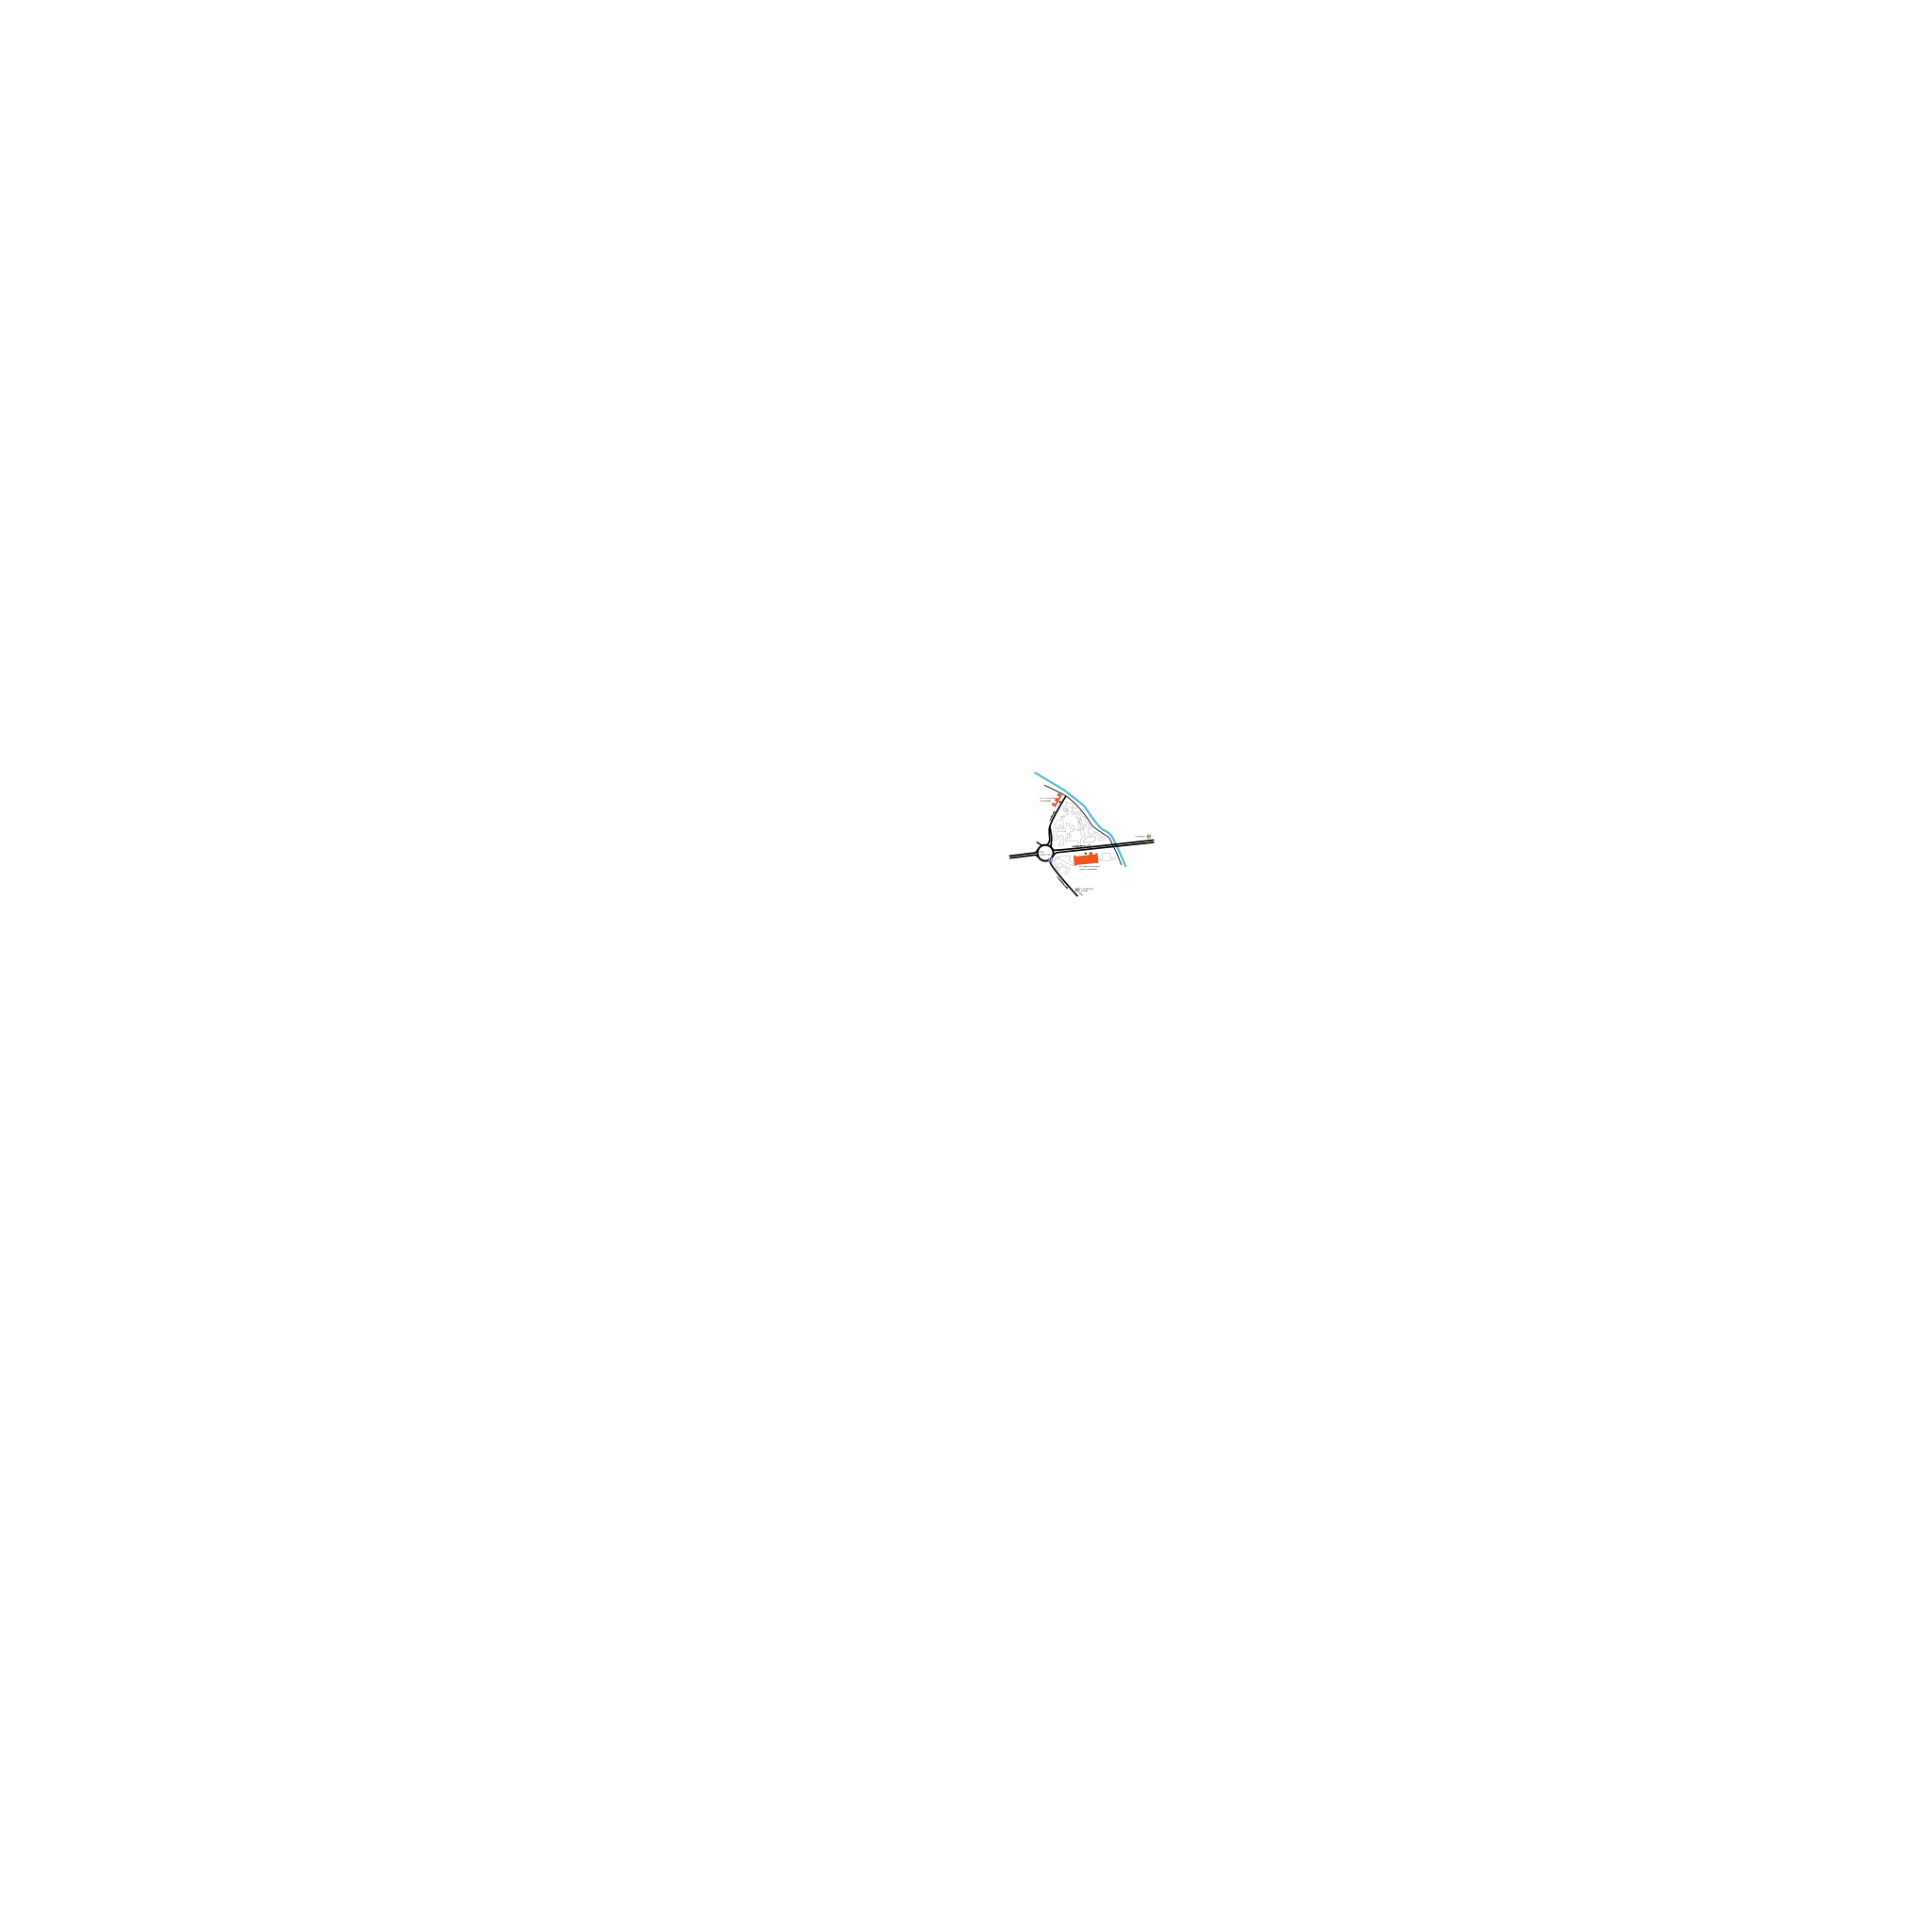
\includegraphics[width=\linewidth]{local_img/maps/RSS_Campus_Map}
\end{figure}

The conference will take place in the main building (building code H) of TU Berlin. The workshops and interactive poster sessions will take place in the building at Marchstra{\ss}e 23 (building code MAR).

\newpage
\phantomsection \section{Floor Plan Building H -- Conference Venue}
Monday, June 24 to Wednesday, June 26
\begin{figure}[h!]
\center
\includegraphics[height=0.8\textheight]{local_img/maps/H_booklet}
\end{figure}

\newpage
\phantomsection \section{Floor Plan Building MAR -- Workshops Venue}
Thursday, June 27 to Friday, June 28

\begin{figure}[h!]
\center
\includegraphics[height=0.8\textheight]{local_img/maps/MAR_booklet}
\end{figure}

\vspace{1.0cm}
{On Thursday, June 27, onsite registration will be held on the ground floor of the MAR building until 10 am.  Afterwards you can register in room MAR 5.032 on the 5th floor.}

\clearpage

\phantomsection \section{Floor Plan Interactive Presentations -- Lichthof}

The numbers indicate monitors for the interactive paper presentations. Please refer to the conference program to find the right monitor for each paper.
\begin{figure}[h!]
\center
\includegraphics[height=0.4\textheight]{local_img/maps/interactive_session}
\end{figure}



\phantomsection \section{Banquet Information}
The Banquet is held on Tuesday, June 25, at the venue \emph{Kater Holzig}, a well-known club in the East of Berlin at the banks of the river Spree. The club is located 600m from the S-train station Jannowitzbr\"ucke. To get there from the conference venue by public transport:
\begin{itemize}
 \item walk eastwards (towards Siegess\"aule and Brandenburg Gate) on \emph{Stra{\ss}e des 17. Juni} to S-train station  \emph{Tiergarten}
 \item take any eastbound S-train (towards Hauptbahnhof, main train station, trains will be headed towards the Northeast at the station) to station \emph{Jannowitzb\"ucke} (6 stops)
 \item follow the map below (ca.~600m). 
\end{itemize}

\label{sec:banquetinfo}
\begin{figure}[h!]
\center
\fbox{\includegraphics[width=3in]{local_img/maps/katerholzig_labeled}}
\end{figure}

After crossing the bridge, turn left through a boarded fence and enter the venue via an unpaved path. When you start wondering whether you are at the right place, you are at the right place.  Just keep on walking.  The address of Kater Holzig is Michaelkirchstra{\ss}e 23; the GPS coordinates are: 52.511283,13.42393. 

The trip takes about 45 minutes. The banquet will begin at 20:00.


\begin{landscape}
\phantomsection \section{Public transport map}
\begin{figure}[h!]
\includegraphics[height=0.9\textwidth, keepaspectratio]{local_img/maps/bvg}
\end{figure}
\end{landscape}


%set back fbox frame
\setlength\fboxrule{0pt}

